\chapter{Opis uporabe programa}


V tem poglavju bo opisana uporaba programa, ki je nastal v okviru te diplomske naloge. Program lahko služi kot učni pripomoček ali pa kot pripomoček za hitro oceno proizvedene električne energije iz bližnjega potoka ali večje reke. Napisan je v programskem jeziku $Javascript$, poleg katerega sem uporabil tudi knjižnici $React$ za prikazovanje uporabniškega vmesnika in $ChartJs$ za risanje diagramov. Sam program je odprto koden in pod MIT licenco, izvorna koda programa pa se nahaja na spletni strani~\cite{SourceCode}.

Za izračun energetskih parametrov hidroelektrarne s programom moramo najprej vnesti podatke o dimenzijah struge vodotoka in povprečnih dnevnih vrednostih pretoka vodotoka za izbrano obdobje. Podatke lahko pridobimo na način, ki je opisan v poglavju~\ref{sec:teorija_pridobitevPodatkov}.




\section{Vnos podatkov}
Na sliki~\ref{fig:opis_frontpage} je viden uporabniški vmesnik, ki se pokaže ob zagonu programa. S pritiskom na ikono v levem zgornjem kotu izberemo in vnesemo datoteko, ki vsebuje podatke o povprečnih dnevnih pretokih vodotoka, ki smo jih dobili iz ARSO-vega arhiva v .csv formatu za izbrano obdobje analize~\cite{Arso}. Primer podatkov v datoteki je prikazan spodaj. Vejica loči datum meritve in povprečni dnevni pretok izbranega vodotoka.

\begin{figure}[htp!]
	\begin{centering}
		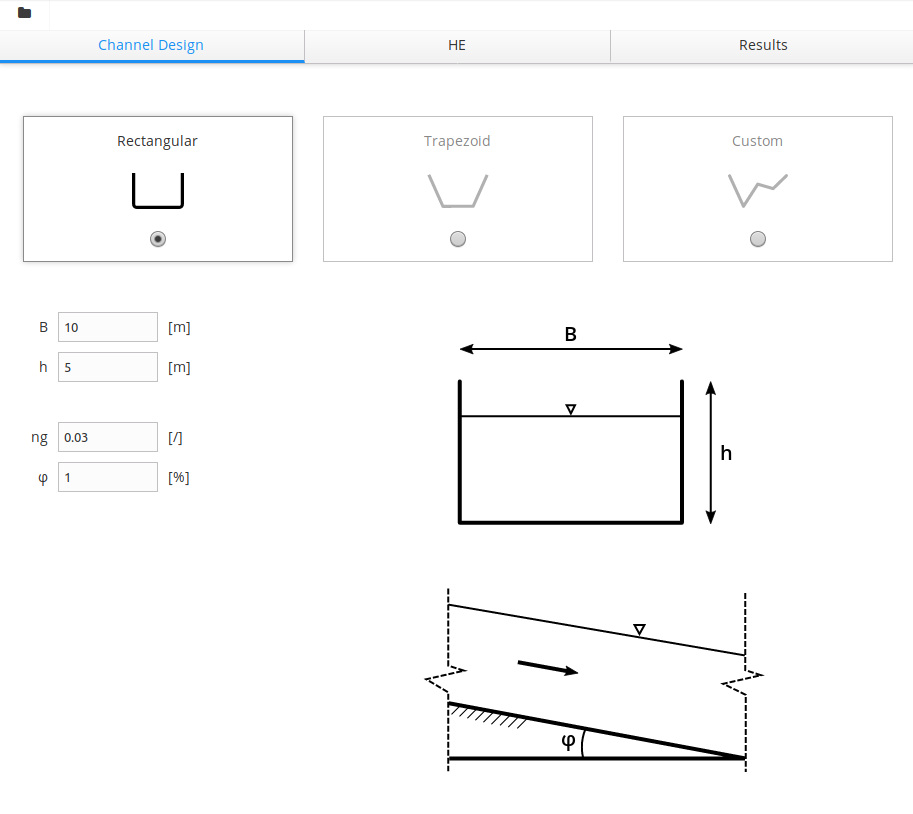
\includegraphics[width=\textwidth]{slike/opis/zagon_programa.png}\caption{Uporabniški vmesnik ob zagonu programa}\label{fig:opis_frontpage}
	\end{centering}
\end{figure}

\begin{center}
01.01.1989,85.1\\
02.01.1989,83.6\\
03.01.1989,85.1\\
04.01.1989,82.1\\
05.01.1989,73.6\\
06.01.1989,69.6\\
07.01.1989,74.9\\
08.01.1989,79.2\\
09.01.1989,80.6\\
10.01.1989,79.2\\
11.01.1989,79.2\\
12.01.1989,79.2\\
itd...\\
\end{center}

Po vnosu podatkov o povprečnih dnevnih pretokih vodotoka, program samodejno analizira podatke o pretokih in v zavihku $Results$ izriše hidrogram in krivuljo trajanja. Primer izpisa hidrološke analize je viden na slikah~\ref{fig:opis_hidrogram} in~\ref{fig:opis_krivuljaTrajanja}. S pritiskom na leto analize, ki se nahaja nad samim diagramom, lahko izbrano leto analize odstranimo oz. filtriramo iz diagrama analize.


\begin{figure}[htp!]
	\begin{centering}
		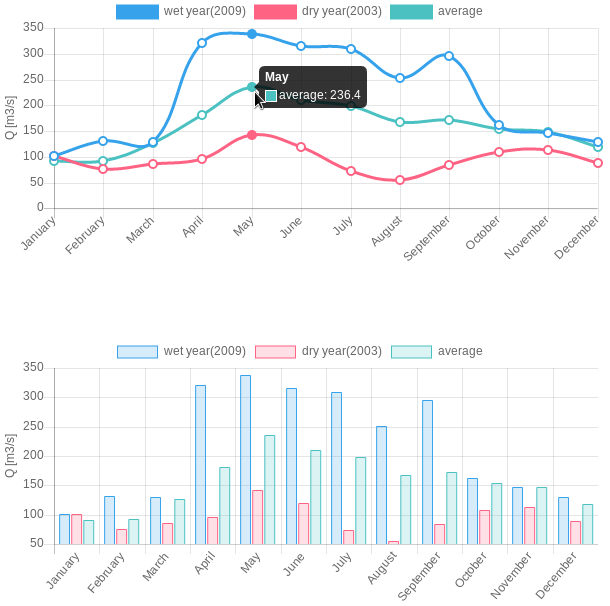
\includegraphics[width=\textwidth]{slike/opis/hidrogram.png}\caption{Primer izračunanega hidrograma v črtnem in stolpičnem diagramu}\label{fig:opis_hidrogram}
	\end{centering}
\end{figure}


\begin{figure}[htp!]
	\begin{centering}
		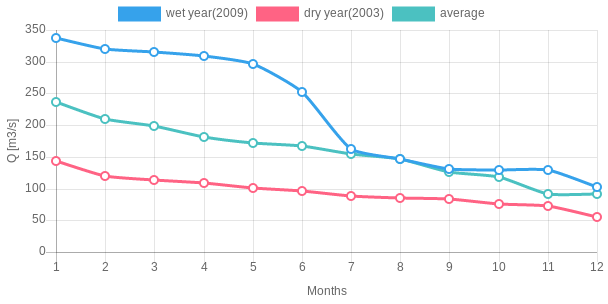
\includegraphics[width=\textwidth]{slike/opis/krivuljaTrajanja.png}\caption{Primer izračunane krivulje trajanja pretokov}\label{fig:opis_krivuljaTrajanja}
	\end{centering}
\end{figure}




\newpage

\section{Izračun konsumpcijske krivulje}\label{sec:izracun}

Za izračun ocene parametrov pretočne hidroelektrarne je ključnega pomena pravilen izračun konsumpcijske krivulje za izbran vodotok, saj se vsi nadaljnji izračuni nanašajo nanj. V tem poglavju bomo na primeru pokazali pravilnost postopka izračuna konsumpcijske krivulje. V ta namen bomo uporabili namišljen primer trapezno oblikovane struge vodotoka prikazane na sliki~\ref{fig:izracun_trapeznaStruga}, z 1\% naklonom struge, višino vode v strugi $h=5m$ in Manningovim koeficientom hrapavosti $n_g = 0,3$.

Rezultate ročnega izračuna bomo primerjali z rezultati ki jih izračuna program po metodi za pravokotno in trapezno oblikovane struge in metodi za izračun pretokov za strugo poljubne oblike opisani v poglavju~\ref{sec:teorija_trapeznaMetoda}  oz.~\ref{sec:teorija_metodaPoljubnaOblika}. Vse mere na spodnji  sliki~\ref{fig:izracun_trapeznaStruga} so v metrih.



\begin{figure}[ht!]
	\begin{centering}
		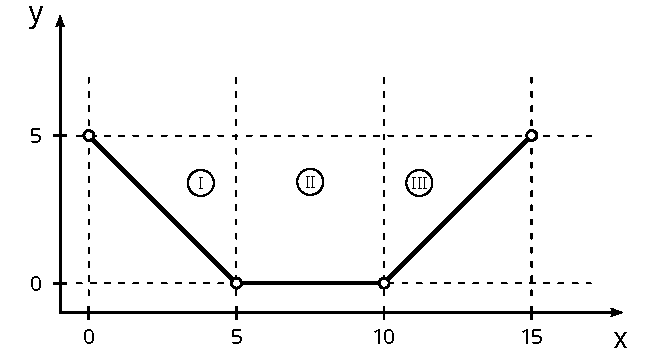
\includegraphics{slike/izracuni/shema_trapezneStruge.pdf}		
		\caption{Shema rečnega korita obravnavanega vodotoka}\label{fig:izracun_trapeznaStruga}
	\end{centering}
\end{figure}




%----------------------------------------------
\section{Izračun parametrov po metodi za pravokotno in trapezno oblikovano strugo vodotoka}\label{sec:izracun_trapeznaMetoda}

V tem poglavju bomo preverili pravilnost delovanja implementiranega algoritma. V ta namen bomo primerjali rezultate ročnega izračuna z rezultati, ki jih izračuna program po metodi za pravokotno in trapezno oblikovane struge opisani v poglavju~\ref{sec:teorija_trapeznaMetoda}.


\subsection{Ročni izračun}
Za izračun pretoka vodotoka pri višini $h=5m$ uporabimo enačbe navedene v poglavju~\ref{sec:teorija_trapeznaMetoda}.
\begin{ceqn}
	\begin{align}
	P(h)&= b + 2 \cdot \sqrt{h^2 + \left(\dfrac{h} {\tan\alpha} \right)^{2}} = 5 + 2 \cdot \sqrt{5^2 + \left(\dfrac{5} {\tan 45} \right)^{2}} = 19,14~m \\
	S(h)&= b \cdot h +  \dfrac{h^{2}}{\tan{\alpha}}   = 5 \cdot 5 +  \dfrac{5^{2}}{\tan{45}}= 50~m^2 \\
	Q(h)&= \dfrac{\sqrt{0,01}}{0,03} \cdot \dfrac{50^{5/3}}{19,1^{2/3}} = 316,1~m^3/s
	\end{align}
\end{ceqn}


\subsection{Izračun s programom}
V program vnesemo podatke o rečnem koritu kot je prikazano na sliki~\ref{fig:trapeznaMetoda_vnosPodatkov}.

\begin{figure}[ht!]
	\begin{centering}
		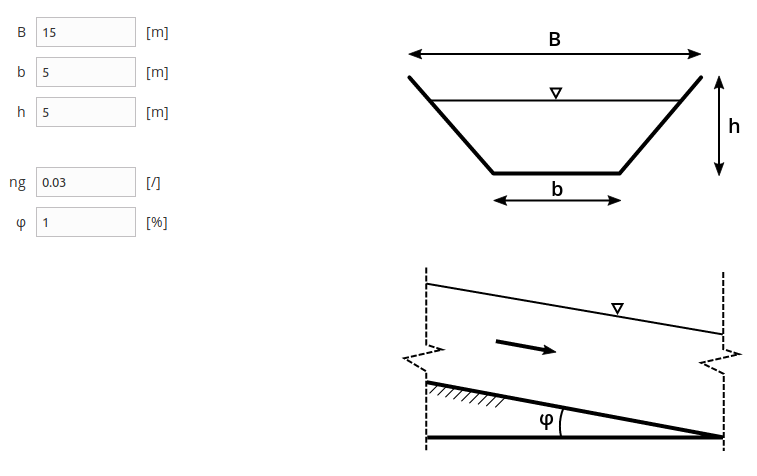
\includegraphics[width=\textwidth]{slike/izracuni/trapeznaStruga.png}		
		\caption{Vnos podatkov v program}\label{fig:trapeznaMetoda_vnosPodatkov}
	\end{centering}
\end{figure}


\begin{figure}[H]
	\begin{centering}
		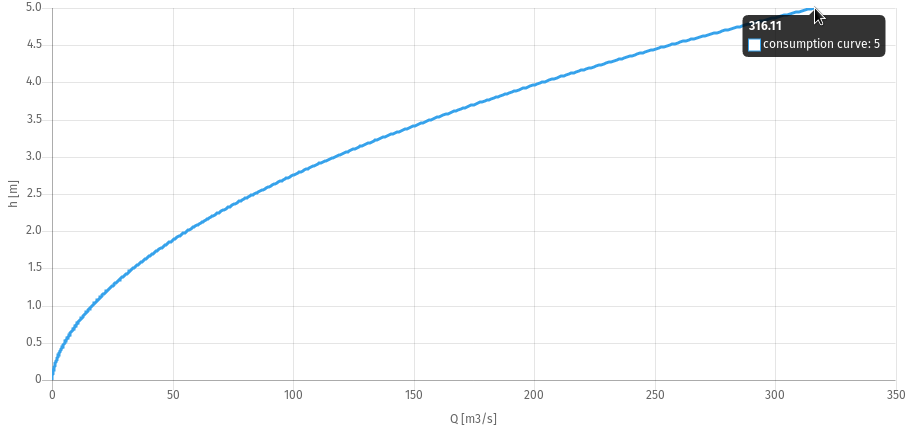
\includegraphics[width=\textwidth]{slike/izracuni/trapezna_konsumpcijska.png}\caption{Konsumpcijska krivulja določena po metodi za pravokotne in trapezno oblikovane struge}\label{fig:trapeznaMetoda_konsumpcijskaKrivulja}
	\end{centering}
\end{figure}



S slike~\ref{fig:trapeznaMetoda_konsumpcijskaKrivulja} lahko pri višini $h=5m$ odčitamo pretok vode v strugi izračunane po metodi za pravokotne in trapezno oblikovane struge $Q = 316,1~m^3/s$. 


%-----------------------------------------------
\section{Izračun parametrov po metodi za strugo poljubne oblike}\label{sec:izracun_numericnaMetoda}

V tem poglavju bomo primerjali rezultate ročno izračunanih parametrov in parametrov izračunanih s programom po metodi za izračun pretoka vode v strugi poljubne oblike opisani v poglavju~\ref{sec:teorija_metodaPoljubnaOblika}.


\subsection{Ročni izračun parametrov hidroelektrarne}\label{sec:izracun_rocno_numericnaMetoda}

Pretoke v strugi vodotoka računamo po odsekih med točkami s katerimi modeliramo strugo vodotoka, pri maksimalni višini $h=5m$.


\begin{enumerate}[I.]
	
	\item Odsek:
	
	\begin{ceqn}
		\begin{align}
		S_I&=\dfrac{5 \cdot 5}{2} = 12,5~m^2\\
		P_I&=\sqrt{5^2 + 5^2} = 7,07~m\\
		\end{align}
	\end{ceqn}
	
	\item Odsek:
	
	\begin{ceqn}
		\begin{align}
		S_{II}&=5\cdot5 = 25 ~m^2\\
		P_{II}&=5~m\\
		\end{align}
	\end{ceqn}
	
	\item Odsek:
	\begin{ceqn}
		\begin{align}
		S_{III}&=S_{I} = 12,5~m^2\\
		P_{III}&=S_{I} = 7,07~m\\
		\end{align}
	\end{ceqn}
	
\end{enumerate}

Skupni pretok pri $h=5 m$ izračunamo kot:

\begin{ceqn}
	\begin{align}
	S_s(h) &= S_{I} + S_{II} + S_{III} = 12,5 + 25 + 12,5 = 50~m^2\\
	P_s(h) &= P_{I} + P_{II} + P_{III} = 7,07 + 5 + 7,07 = 19,14~m\\
	Q_s(h)&= \dfrac{\sqrt{0,01}}{0,03} \cdot \dfrac{50^{5/3}}{19,14^{2/3}} = 316,1~m^3/s
	\end{align}
\end{ceqn}




\subsection{Izračun parametrov hidroelektrarne s programom}

S pomočjo uporabniškega vmesnika v koordinatni sistem vnašamo serijo točk, s katerimi modeliramo robove izbrane struge. V našem primeru so vrednosti koeficientov za vse odseke rečne struge enake.

\begin{figure}[H]
	\begin{centering}
		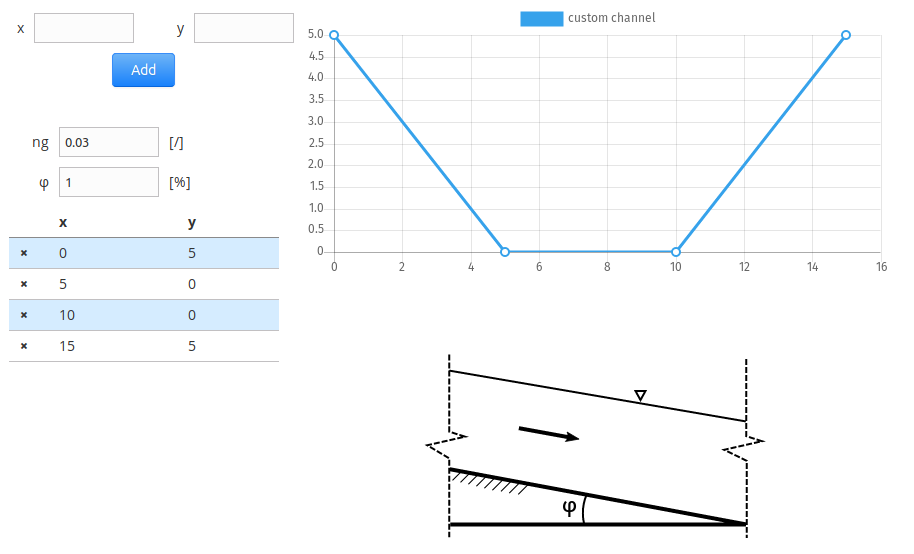
\includegraphics[width=\textwidth]{slike/izracuni/poljubna_struga.png}\caption{Vnos podatkov v program}\label{fig:modeliranjeStruge}
	\end{centering}
\end{figure}

% H forces image to stand here on this place -> pushes text below
\begin{figure}[H]
	\begin{centering}
		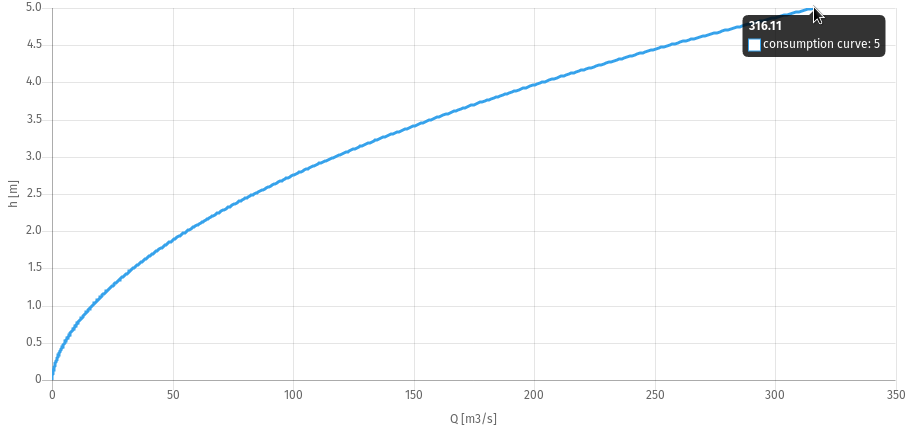
\includegraphics[width=\textwidth]{slike/izracuni/poljubna_konsumpcijska.png}\caption{Graf konsumpcijske krivulje izračunani po metodi za poljubno oblikovane struge}\label{fig:custom_konsumpcijskaKrivulja}
	\end{centering}
\end{figure}


Z grafa konsumpcijske krivulje \ref{fig:custom_konsumpcijskaKrivulja} pri višini $h = 5 m$ lahko odčitamo pretok $Q=316,1~m^3/s$, ki je enak rezultatu ročnega izračuna v poglavju~\ref{sec:izracun_rocno_numericnaMetoda} in rezultatu dobljenem po metodi za pravokotne in trapezno oblikovane struge v poglavju~\ref{sec:izracun_trapeznaMetoda}. S tem smo dokazali pravilnost numeričnega algoritma za izračun točk konsumpcijske krivulje za poljubno oblikovano strugo vodotoka.




%----------------------------------------------
%FIXME: add content
%\section{Rezultati izračuna konsumpcijske krivulje} \label{sec:opis_rezultatIzracuna}
%V poglavjih ~\ref{sec:izracun_trapeznaMetoda} in ~\ref{sec:izracun_numericnaMetoda} smo preverili, da sta rezultata ročnega izračuna in izračuna s programom enaka.


